\section{Discussion}
\label{sec:discussion}

In Section \ref{sec:method}, we have proposed a new coverage notion that
is more practical to use. Although the minimality of $SOS$ makes $\psi_{sos}$ accurate 
in terms of both preserving provability and not having false positives, as discussed, the exact implementation of $\psi_{sos}$ is based on the \ucbfalg algorithm, which is as nearly expensive as the \mustalg algorithm for $\psi_{sm}$.
 To alleviate this issue, we came up with an efficient implementation for $\psi_{sos}$, i.e. \ucalg \cite{Ghass16}, 
 which is an over-approximation and might not be always accurate in terms of minimality. 
 However, the idea of IVCs or support sets makes
it possible to have other coverage metrics in formal verification, which is beneficial, as with testing, because if a
coverage notion is an over-approximation, when the coverage
 is high, it does not necessarily mean the quality of
 the specification (or test suite) is high, or when it is an under-approximation, a low coverage does not always mean the specification is of poor quality.

 As mentioned in Section \ref{sec:impl}, support sets are derived from inductive invariants; in other words, they are built upon the proof of the validity of a given property. One interesting fact about proofs
  is that a given property could be proved from different proof paths. That's why we defined $ASOS(r)$ in Section \ref{sec:background}. The $ASOS$ set gives a clear picture of various ways a property is satisfied. By getting all the support sets for all requirements of the system and categorizing them, one can find if there are target artifacts that do not trace to any requirement: set $\bigcap \{IRR (r) | r \in \Delta \}$.  If this set is non-empty, it is a possible indication of ``gold plating" or missing requirements. That is to say, it helps to assess if the requirements of the system describe all the behaviors of the system. Being able to measure the coverage of requirements over the model is crucial in the safety critical system domain.

Very recent, as yet unpublished, work has focused on the
generation of all support sets (IVC sets), whose preliminary evaluation
shows the overhead in discovering all support sets is a linear in the
number of unique support set in the problem multiplied by the cost
for finding a proof for a single support set. For complex models, such
as the ones described in \cite {QFCS15:backes} and \cite{hilt2013}, it has been possible to
find $ASOS$ for individual properties in a matter of minutes.
Based on our preliminary results we expect computing $ASOS$ to be computationally feasible for complex models. In
addition, we believe that it is possible to use the information
from the set of all IVCs to more efficiently produce minimal
IVCs than the \ucbfalg algorithm.

Since the primary goal of
 this paper has been to provide a complementary coverage notion in
  formal verification, having an efficient technique to practically compute $ASOS$, it is worth exploring other possible notions based on the idea of provability and $ASOS$.

\begin{definition} {\emph{Complementary coverage notion 1:}}
  \label{def:comp-1}
   $ R = \bigwedge_{i} {r_i \in \Delta}, \varphi \in \Gamma,  \psi (R) \preccurlyeq \varphi$ iff $ \exists S
   \in ASOS(R)$. $\varphi \in S$.
\end{definition}

\begin{figure}
\begin{center}
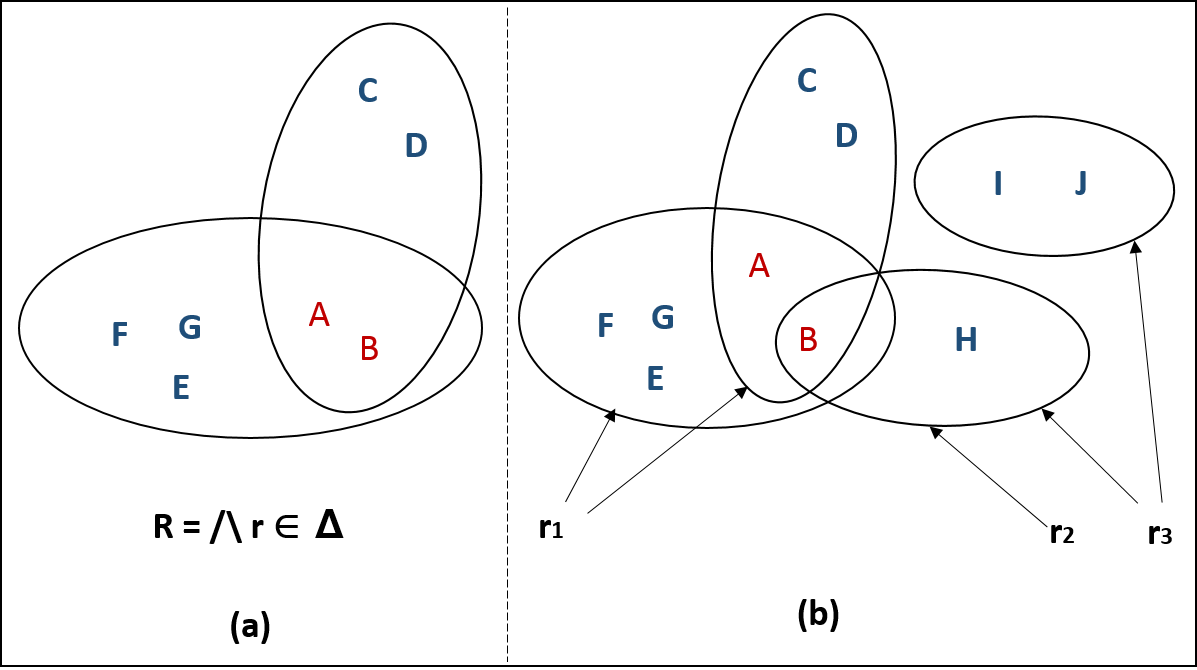
\includegraphics[width=\columnwidth]{figs/disc.png}
\vspace{-0.1in}
\caption{A visual example to illustrate other coverage notions with $ASOS$}\label{fig:disc}
\end{center}
\end{figure}

Consider Fig. \ref{fig:disc} (a); it represents two distinct support sets for $ R = \bigwedge_{i} {r_i \in \Delta}$. If \ucalg returns support set $\{ A, B, C, D\}$, then $\psi_{sos}$ will
report elements $\{ F, G, H\}$ as uncovered, while they are not. However,
the coverage function proposed in Definition \ref{def:comp-1} will mark all the elements in the example as covered.

\begin{definition} {\emph{Complementary coverage notion 2:}}
  \label{def:comp-2}
   $\forall \varphi \in \Gamma,  \psi (R) \preccurlyeq \varphi$ iff $ \exists S
   \in ASOS(r), r \in \Delta$. $\varphi \in S$.
\end{definition}

Another example provided in Fig. \ref{fig:disc} (b) shows a design with
three requirements $\{ r_1, r_2, r_3\}$. As you can see, each requirement points to its
own support sets; for example, $r_3$ has two support sets,
which means $ASOS(r_3) = \{ \{B, H\}, \{I, J\}\}$. In this example,
function $\psi_{sos}$ marks $\{I, J\}$ as uncovered, while they are actually covered in a way by $r_3$.
However, Definition \ref{def:comp-2} will consider them as covered by $r_3$.
Note that $\psi_{sm}$ is even much harder to satisfy; for instance, in Fig. \ref{fig:disc},
it will only consider $\{ A, B\}$ as covered.

These two definitions proposed in this section are computationally much more expensive than the metric in Definition \ref{def:coverage-ivc}. However, they are easier to satisfy. A preliminary evaluation shows that they are as nearly expensive as the metric computed by the \mustalg algorithm for Definition \ref{def:coverage1}.
In terms of preserving provability, a set of design elements marked as covered by Definition \ref{def:comp-1} and \ref{def:comp-2} are
sufficient to reconstruct the proof of any requirement in $\Delta$.

